
\section{ Experiment}

\noindent We used the map of Helsinki in our simulator to evaluate the performance of the proposed ACP. We also compare it to Binary Spray and Wait (BSW) protocol \cite{C31}, distributed social based location privacy protocol (SLPD) \cite{C16} and our Multi-Hop Location-Privacy Protection (MHLPP). We simulated the continuous movement of users along streets on the map with one LBSP, fixed at a random location on the map.

For each user, we associate a random social value between 0 - 100\%, each corresponding to other users. Since each social value is assigned with equal probability, we can compute the expected number of friends of a user. If a user whose social value is larger than 85\% is called a friend and there are \textit{n} users in the network, there are $n\times \left(1-85\%\right)$ friends.

The Shortest Path Map-Based Movement (SPMBM) \cite{C35} is used in our experiment. For each experiment, we give the simulator a random seed so that it can generate a pseudo-random number based on the seed. Therefore, all the factors including users' speed and locations are the same if two experiments have the same random seed. All four protocols are tested using the same set of random seeds.

Before each experiment, the simulator runs for 800 seconds (simulator time). Then we pick 100 users out of 126 users randomly, and each of them sends a query to the LBSP. Tests last for about 20 minutes (simulator time). 


\subsection{  Average Query Success Ratio}

\noindent The query success ratio is the percentage of delivered queries among some attempts. Since users sending 100 queries in each experiment, if $s$ queries are delivered to the LBSP at time $t$, the query success ratio of time $t$ is $s\%$.

As shown in Figure \ref{fig:AverageQuerySuccessRatio10}, we compare the average query success ratio of the four protocols with 5 kinds of communication radius (10, 30, 50, 70 and 90 meters). We observe that the ACP and the BSW get a high query success ratio, while the MHLPP and the SLPD are lower than the previous two protocols. The BSW is the highest one because it is a no-privacy protocol. The ACP is just a little lower than BSW, because the query delivery process of the ACP is almost the same as that of BSW. Since users of ACP must wait for available appointment cards, they cost more time to initial their queries. However, the ACP and the BSW are at the same level, comparing to the other two protocols. The MHLPP and the SLPD need to find friends to obfuscate their queries, which baffles their delivery process.

\begin{figure} [H]
  \centering 
  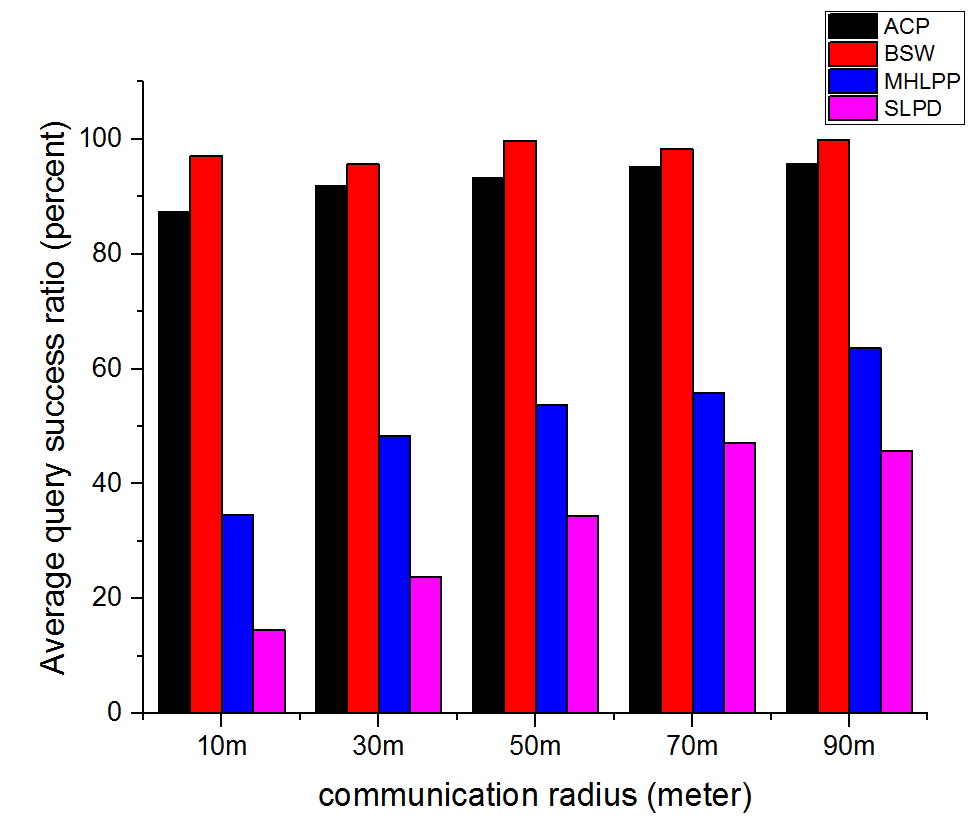
\includegraphics[width=4.0in]{figures/F414AverageQuerySuccessRatio10minutes.png}
  \caption{Average Query Success Ratio (10 minutes)} 
  \label{fig:AverageQuerySuccessRatio10} %% label for entire figure 
\end{figure}

The experiment results when we test 20 minutes is shown in Figure \ref{fig:AverageQuerySuccessRatio20}. Comparing to the average query success ratio at 10 minutes, the MHLPP and the SLPD achieve much higher success ratio after 20 minutes than at 10 minutes. That is because it cost them so much time in their obfuscation phases when they need to find friends. In fact, some of the queries of the MHLPP and the SLPD still do not finish their obfuscation phase at 20 minutes.

\begin{figure} [H]
  \centering 
  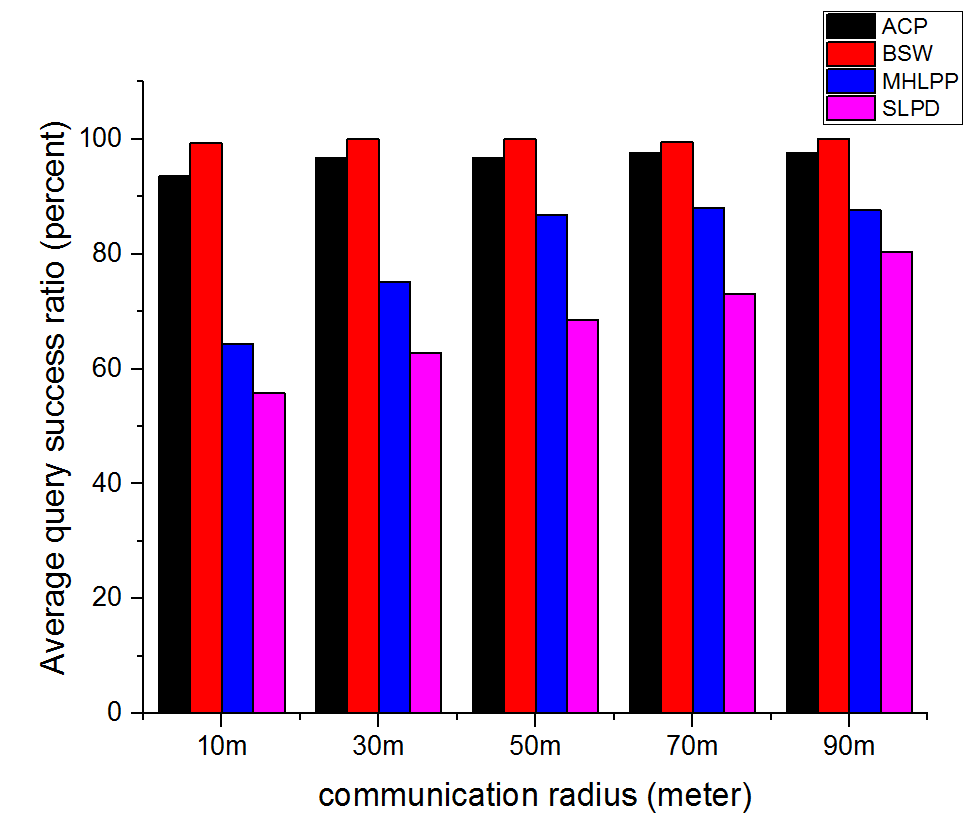
\includegraphics[width=4.0in]{figures/F415AverageQuerySuccessRatio20minutes.png}
  \caption{Average Query Success Ratio (20 minutes)} 
  \label{fig:AverageQuerySuccessRatio20} %% label for entire figure 
\end{figure}

The communication radius can influence the success ratio. In most of the cases, the success ratio rises when we increase the communication radius, and its influence is especially evident under 50 meters. A large communication radius makes it easy for users to encounter others, which is good for them to forward queries. However, a user who is so far away from the destination does not want the intermediates of his query encounters many users nearby. Because all users who carry copies of that query are near the sender instead of the destination, which decreases their query success ratio. Therefore, when the communication radius reaches 70 meters, the success ratios almost stay at the same level.

In Figure \ref{fig:F416AverageQuerySuccessRatioWith50MetersCommunicationRatio}, we observe that the ACP and the BSW have better convergence speed than the MHLPP and the SLPD. In other words, the former two protocols have a faster speed to approach the 100\% query success ratio than the latter two. At the very beginning, the ACP even has a little higher success ratio than the BSW. Because the ACP users need ready appointment card, and most of the users get their first ready appointment cards at places where there are many users. Therefore, users rarely generate query near the edges of the map at the beginning, which facilitates their queries delivery process. For example, if a user generates his query at the edge of the map, the copies of this query might be sent to users who are also at the edge, and it takes more time for them to deliver the query. If the user does not generate his query until he arrives a place nearer the center, the copies of this query will be carried by the users in the center with higher probability.

\begin{figure} [hbtp]
  \centering 
  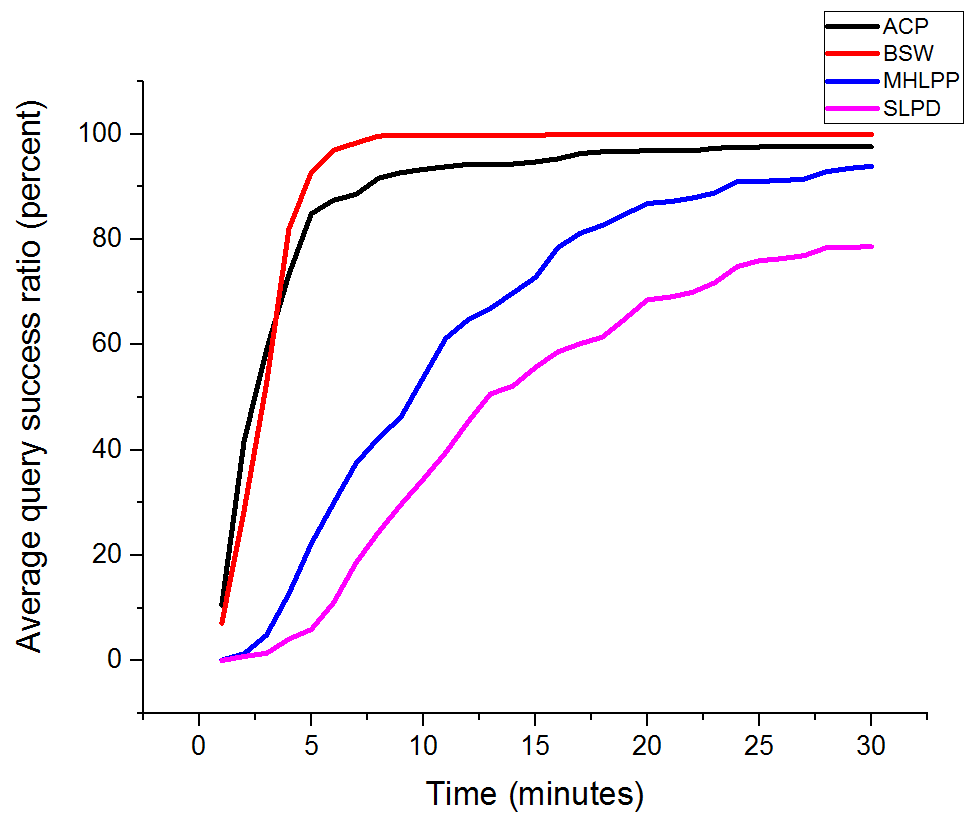
\includegraphics[width=4.0in]{figures/F416AverageQuerySuccessRatioWith50MetersCommunicationRatio.png}
  \caption{Average Query Success Ratio With 50-Meters Communication Ratio} 
  \label{fig:F416AverageQuerySuccessRatioWith50MetersCommunicationRatio} %% label for entire figure 
\end{figure}

\subsection{ Average Reply Success Ratio}

\noindent When the LBSP receives a query, it sends a reply to the requester. If the reply arrives the original requester before the test ends, we view it as a success; otherwise, the reply is failed. There are two reasons for the failure of replies: 1) the query is not delivered to the LBSP successfully; 2) the query costs too much time so that the reply has no time to be delivered; 3) The route of the reply is too long. Since there are 100 queries in each experiment, the number of replies should be equal to 100. 

In Figure \ref{fig:F417AverageReplySuccessRatioWith50MetersCommunicationRatio}, the BSW has a significant and reasonable higher success ratio than all other protocols, because it is a no-privacy protocol. The ACP is higher than the MHLPP and the SLPD, but its advantage is not as large as that in the query process. In fact, the reply process of the MHLPP and the SLPD are simpler than that of the ACP, but the ACP saves so much time in its query process that it earns a better reply success ratio than the other two.

\begin{figure} [hbtp]
  \centering 
  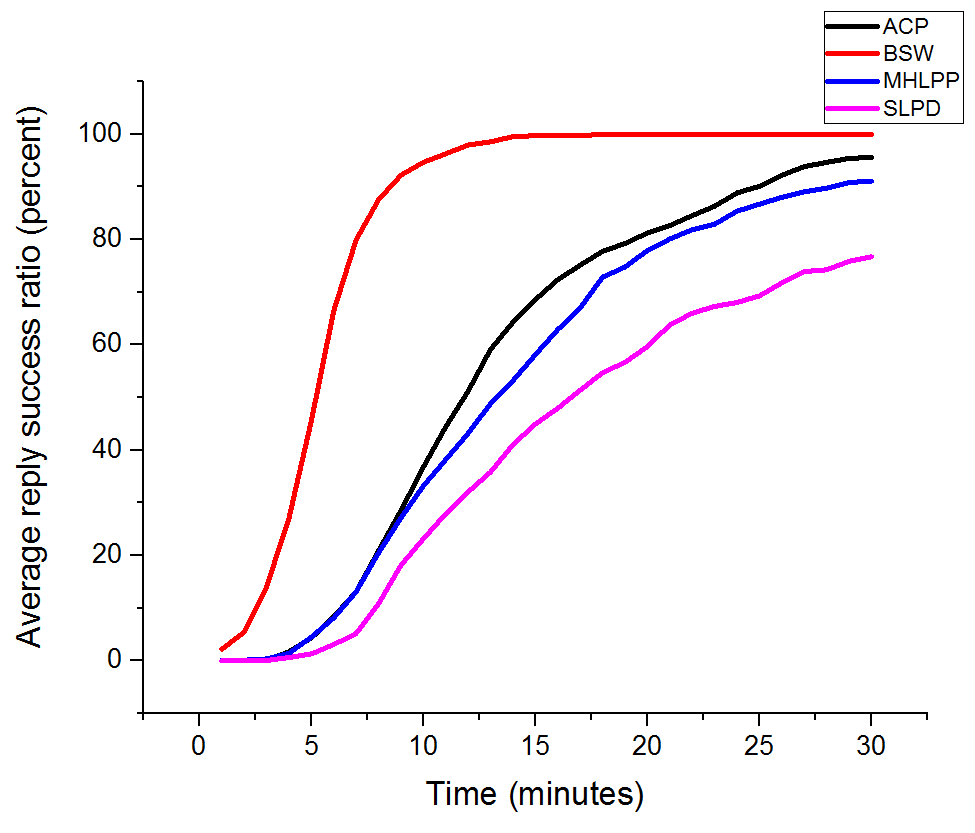
\includegraphics[width=4.0in]{figures/F417AverageReplySuccessRatioWith50MetersCommunicationRatio.png}
  \caption{Average Reply Success Ratio With 50-Meters Communication Ratio} 
  \label{fig:F417AverageReplySuccessRatioWith50MetersCommunicationRatio} %% label for entire figure 
\end{figure}

\subsection{ Total Number of Query Relays}

\noindent The query delivery processes of all the four protocols use the BSW protocol, and the BSW makes copies for queries and gives half of the copies to any users it encounters. That is a significant cost for the network, so we use the number of query relaying (QR) to evaluate that cost. The QR is initialized as zero at the beginning of the test. When a user relay a (or several) copies of a query, we increase QR by 1. For example, in the SLPD, there are two phases: the obfuscation phase and the free phase. In the obfuscation phase, a query is forwarded among one-hop friends for $k$ times. After that, it is forwarded by the BSW protocol. The BSW protocol makes $c$ copies of the query and gives half of the copies to any encountering users. Then QR should be about $k+c$. Since a user gives all its copies to the destination if he encounters the destination at once, the QR may be smaller. The smaller that number is, the smaller cost of the network is. Since there are 100 queries, we divide QR by 100 to get an average value. 

In Figure \ref{fig:F418AverageTotalNumberofForwardingQueriesAt20Minutes}, we compare QR with four protocols. We observe that all the four protocols are at a similar level, the BSW and the ACP is a little lower than the other two. For the ACP and the BSW, they deliver queries so fast that users who carry more than one copies give all their copies to the destination before they send these copies to different users separately. As a result, many copies have no chance to be forwarded, which decreases the cost. While the MHLPP and the SLPD have obfuscation phases, the queries start to be delivered freely (in a BSW way) at a random place where might be so far away from the destination, so that almost all copies can be forwarded respectively.

\begin{figure} [hbtp]
  \centering 
  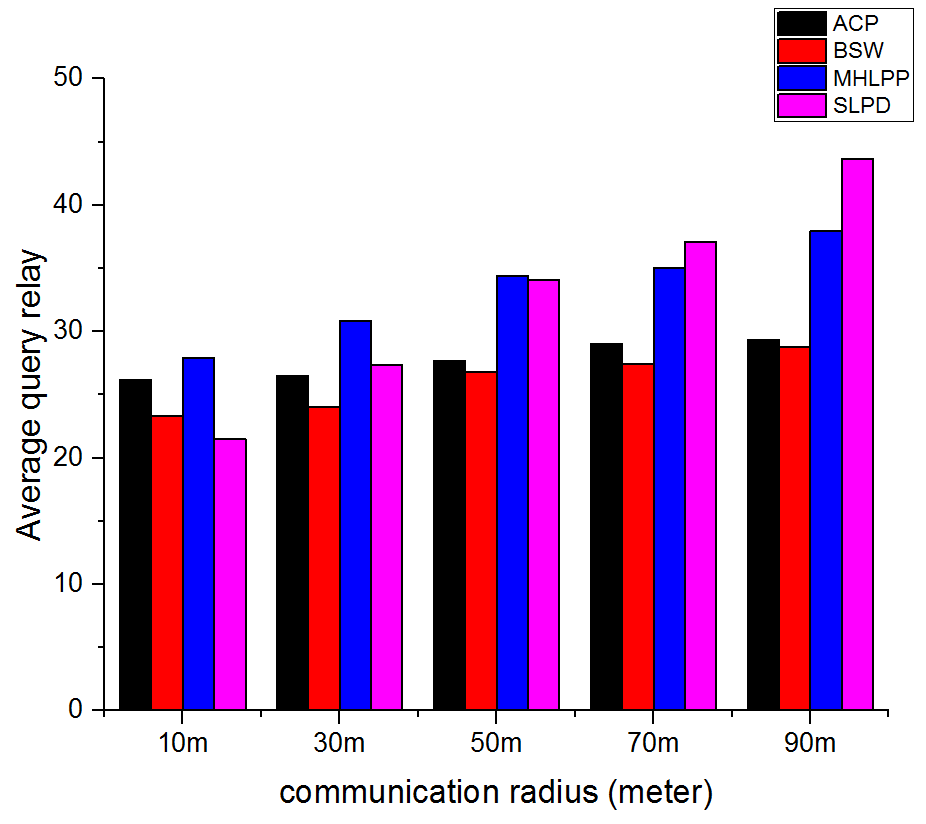
\includegraphics[width=4.0in]{figures/F418AverageTotalNumberofForwardingQueriesAt20Minutes.png}
  \caption{Average Total Number of Forwarding Queries At 20 Minutes} 
  \label{fig:F418AverageTotalNumberofForwardingQueriesAt20Minutes} %% label for entire figure 
\end{figure}

The communication radius affects the total number of the forwarding queries, especially for the MHLPP and the SLPD. Those two protocols can finish their obfuscation phase more quickly which a larger communication radius, so that more queries can be forwarded freely (in the BSW way), which makes their QR larger.

\subsection{ Memory Cost}

\noindent We count the number of queries carried by each user to evaluate the memory cost of the four protocols. Several copies of a query are counted for only once.

In the Figure \ref{fig:F419AverageQueryBufferNeededAt20Minutes}, we compare the number of queries per user with the four protocols at 20 minutes. We observe that the BSW is the highest in most of the cases and the ACP always stays at a similar level as the BSW. The data of other two protocols (the MHLPP and the SLPD) increase as the communication radius. The MHLPP even excesses the BSW when the communication radius is 90 meters. The reason is that quite a number of the BSW and the ACP users forward their copies to the destination so that there is no copy with them at 20 minutes, while the rest of them cannot forward their copies to the destination even given a large communication radius. At the same time, the number of the other two protocol's free phase queries is significantly influenced by the communication radius. The more queries are in the free phase; the more copies are in the network.

\begin{figure} [hbtp]
  \centering 
  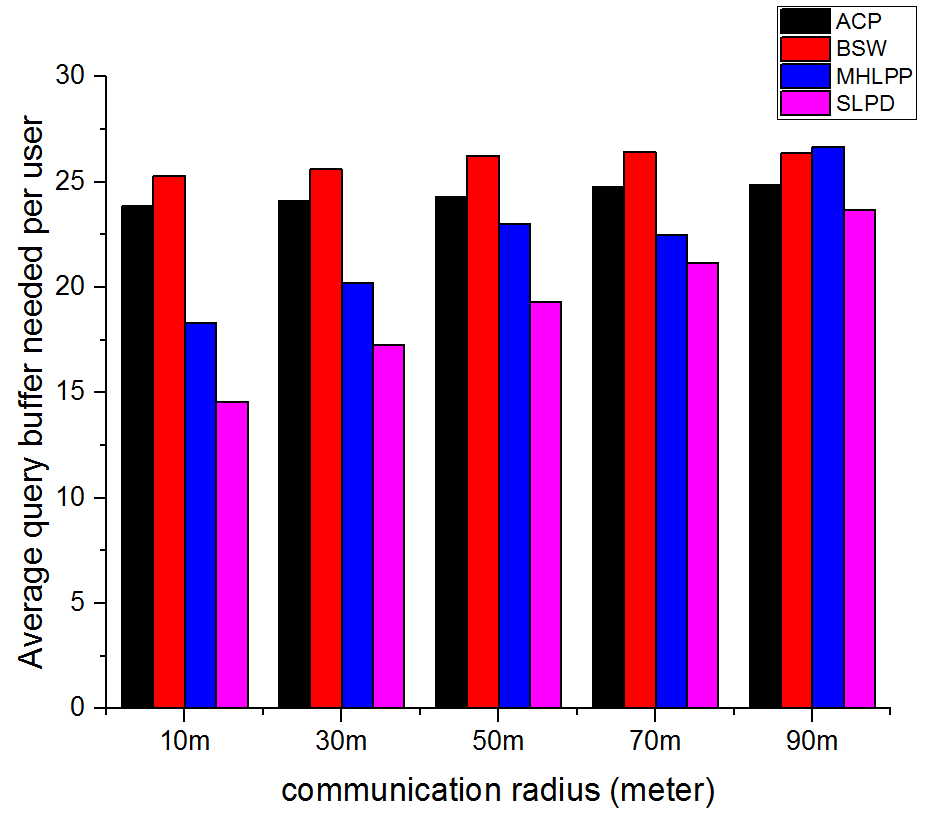
\includegraphics[width=4.0in]{figures/F419AverageQueryBufferNeededAt20Minutes.png}
  \caption{Average Query Buffer Needed At 20 Minutes} 
  \label{fig:F419AverageQueryBufferNeededAt20Minutes} %% label for entire figure 
\end{figure}

The Figure \ref{fig:F420AverageNumberofCarriedQueriesPerUser} shows the average number of queries which are carrying by users when the communication radius is 10, 50 and 90 meters. The curves of the ACP and the BSW rise sharply at the beginning and then become flat, while those of the MHLPP and the SLPD rise smoothly and continuously. 

\begin{figure} [hbtp]
  \centering 
  \subfigure[communication radius is equal to 10 meters]{ 
    \label{fig:F420AverageNumberofCarriedQueriesPerUser:a} %% label for first subfigure 
    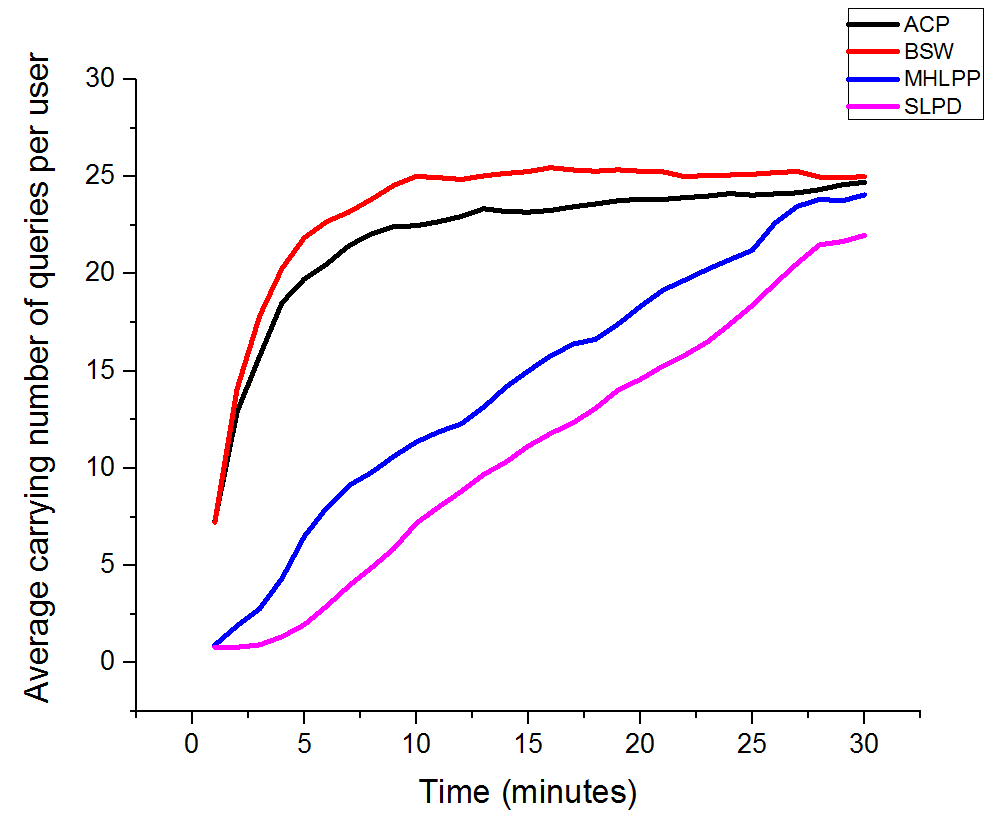
\includegraphics[width=3.0in]{figures/F420AverageNumberofCarriedQueriesPerUser10.png}} 
  \hspace{1in} 
  \subfigure[communication radius is equal to 50 meters]{ 
    \label{fig:AverageNumberofCarriedQueriesPerUser:b} %% label for second subfigure 
    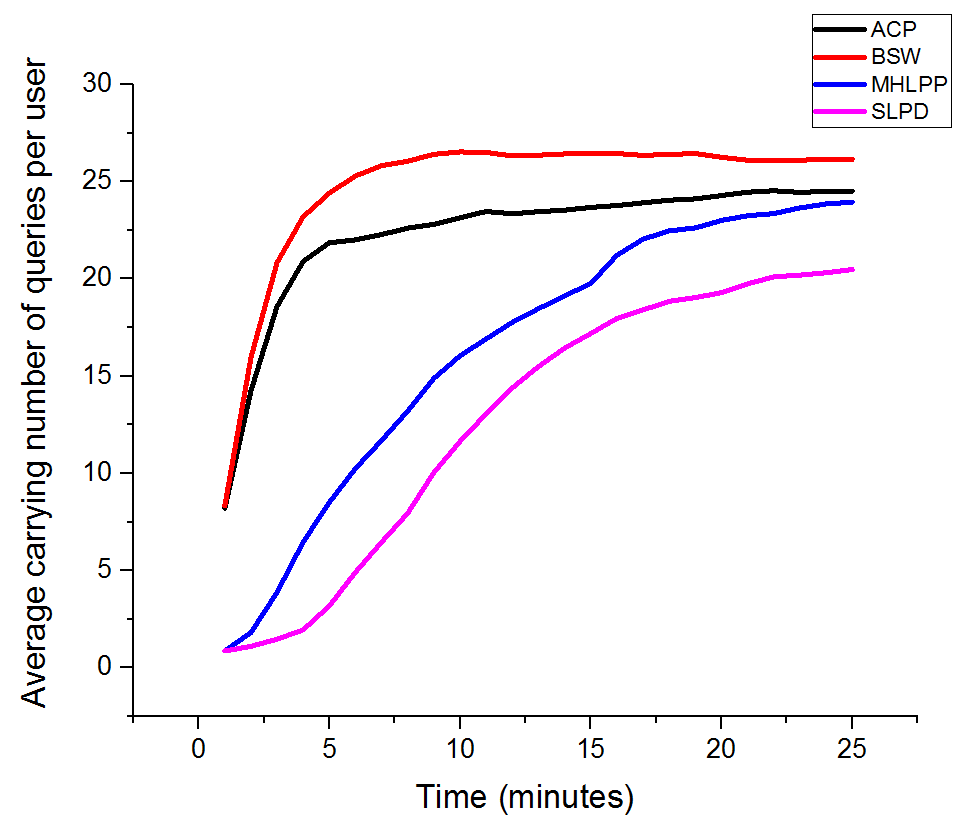
\includegraphics[width=3.0in]{figures/F420AverageNumberofCarriedQueriesPerUser50.png}}
  \hspace{1in} 
  \subfigure[communication radius is equal to 90 meters]{ 
    \label{fig:AverageNumberofCarriedQueriesPerUser:c} %% label for second subfigure 
    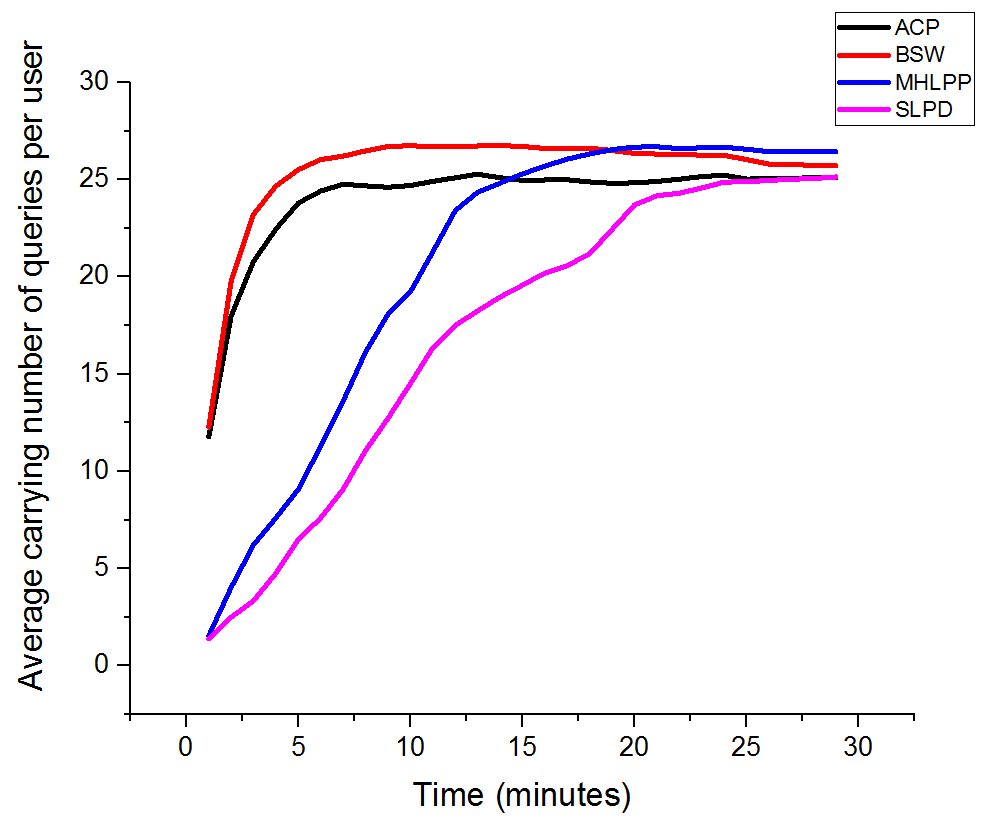
\includegraphics[width=3.0in]{figures/F420AverageNumberofCarriedQueriesPerUser90.png}}
  \caption{Average Number of Carried Queries Per User} 
  \label{fig:F420AverageNumberofCarriedQueriesPerUser} %% label for entire figure 
\end{figure}

\subsection{ Distributing Appointment Cards}

\noindent Exchanging appointment cards is a feature of the ACP, which imports burden into the network. We count the number of exchanging appointment cards per minute to evaluate the extra cost of the ACP.

In Figure \ref{fig:F422AverageNumberofExchangingACsPerMinute}, we count the total number of exchanging ACs in the whole network. For example, if a user Alice encounters another user Bob, the total of exchanging ACs processes increases by one when Alice exchanges any ACs to Bob. We count the number of those exchanging processes occur per minute. As shown in the figure, the exchanging processes do not occur frequently, but about 2 times per minutes. Since the size of an appointment card is small, it does not cost the network many resources. At the same time, users can get many appointment cards to help them send queries, as shown in Figure \ref{fig:F421AverageNumberofReadyACsPerUser}. The number of ready ACs per user is raising smoothly and steadily. 

\begin{figure} [hbtp]
  \centering 
  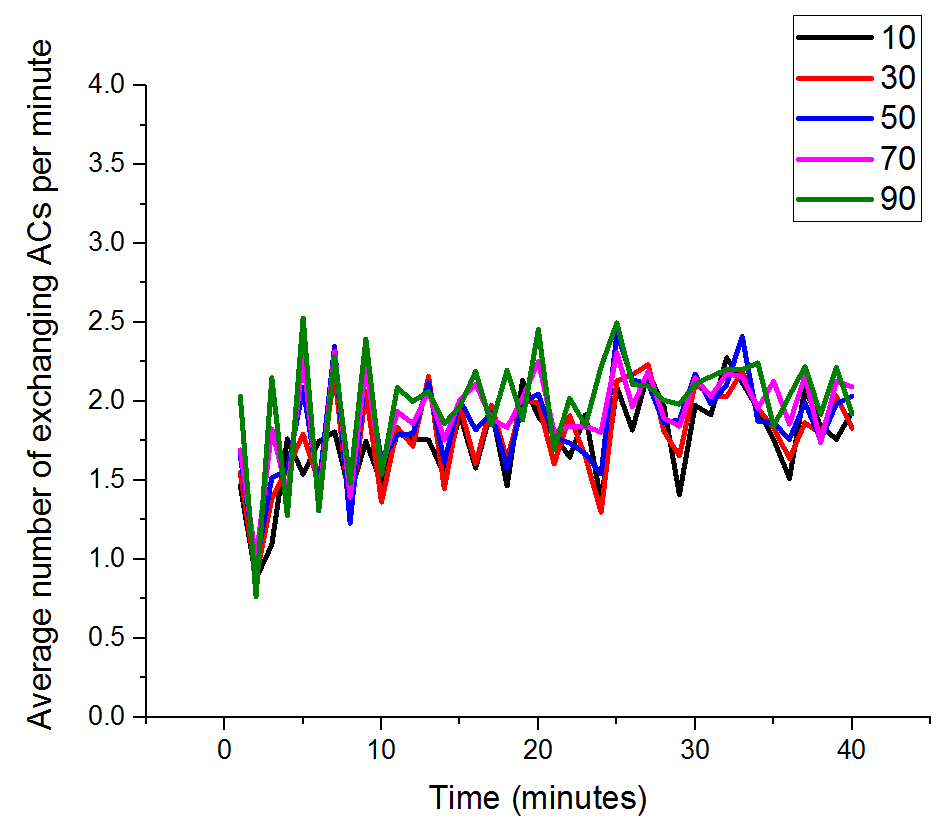
\includegraphics[width=4.0in]{figures/F422AverageNumberofExchangingACsPerMinute.png}
  \caption{Average Number of Exchanging ACs Per Minute} 
  \label{fig:F422AverageNumberofExchangingACsPerMinute} %% label for entire figure 
\end{figure}

\begin{figure} [hbtp]
  \centering 
  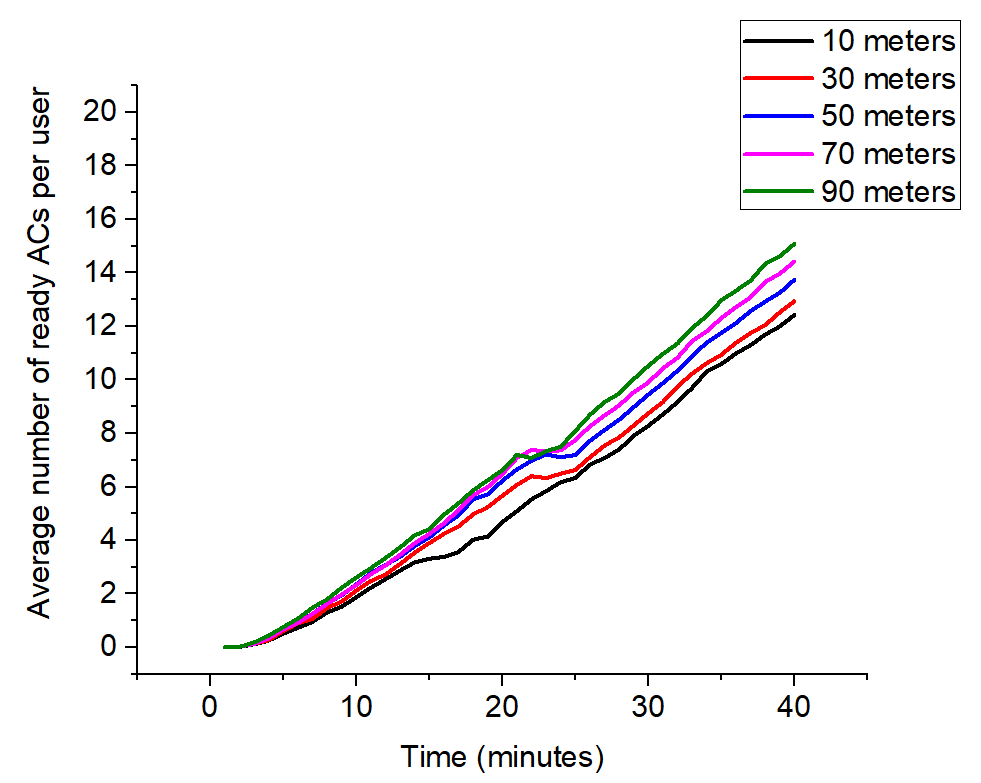
\includegraphics[width=4.0in]{figures/F421AverageNumberofReadyACsPerUser.png}
  \caption{Average Number of Ready ACs Per User} 
  \label{fig:F421AverageNumberofReadyACsPerUser} %% label for entire figure 
\end{figure}


